\title{Pendolo invertito su rotaia}
\maketitle
\label{sec:pic}

\paragraph{Introduzione.}
In questo capitolo sviluppo il modello del sistema e sviluppo due strategie di controllo
basate su quanto ho detto nei capitoli~\ref{sec:linear-control} e~\ref{sec:nonlinear-control}. Mostro poi il sistema reale che ho costruito e su cui si basa il modello.
Concludo illustrando un modo per ottenere alcuni parametri non misurabili
ditettamente.
 
\section{Obiettivi}
Il pendolo invertito su rotaia è un sistema che,
sebbene sia facile da modellare, presenta alcune
caratteristiche che rendono interessante studiarne la
controllabilità.
Il sistema ha due punti di equilibrio; è
\emph{non lineare} e \emph{sottoattuato} (ovvero, un solo controllo
deve controllare due gradi di libertà).
Lo studio che sviluppo in questo capitolo ha il duplice obiettivo di:
\begin{enumerate}
    \item trovare una strategia per stabilizzare il pendolo attorno al punto di equilibrio instabile, in modo che sia resistente alle perturbazioni (\emph{strategia di stabilizzazione}),
    \item trovare una strategia per portare il pendolo in prossimità del punto di equilibrio instabile, partendo dalla configurazione stabile (\emph{strategia di swing-up}).
\end{enumerate}
Applicherò poi questo studio ad un sistema reale che ho costruito, 
in modo da confrontare i risultati teorici con quelli pratici.
\section{Modello del sistema}
Il sistema consiste in un pendolo rigido, libero di ruotare e vincolato a muoversi lungo una rotaia rettilinea tramite un carrello.
L'unico controllo che ho sul sistema è
una forza applicata sul carrello lungo la direzione della rotaia,
così come è mostrato in figura~\ref{fig:pic}.
Io sono interessato
ad applicare questo studio nel mondo reale, quindi devo tenere
in considerazione che la forza è generata da un motore in risposta
a un segnale di input.
Il motore che prendo in considerazione è un motore elettrico
spazzolato. Visto che il motore è un sistema dinamico in sé,
è conveniente modellarlo separatamente rispetto al sistema
carrello-pendolo.
In figura~\ref{fig:pic-real} è
mostrato uno schema del sistema reale.

\begin{figure}[h]
    \centering
    \begin{subfigure}[b]{0.4\textwidth}
        \centering
        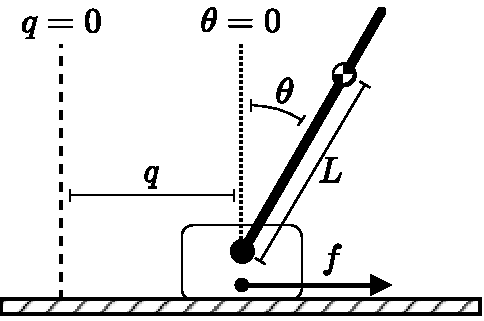
\includegraphics[width=\textwidth]{assets/pic}
        \caption{Schema ideale del sistema. La forza di controllo esterna
        agisce direttamente sul carrello, nella direzione dello scorrimento.}
        \label{fig:pic}
    \end{subfigure}
    \hfill
    \begin{subfigure}[b]{0.48\textwidth}
        \centering
        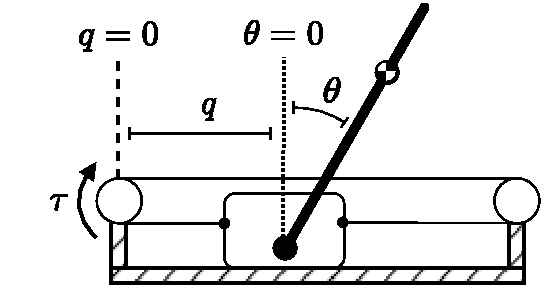
\includegraphics[width=\textwidth]{assets/pic-real}
        \caption{Schema reale del sistema. La forza di controllo viene
        generata da un motore e trasferita al carrello con una cinghia.}
        \label{fig:pic-real}
    \end{subfigure}
    \caption{Schema del sistema ideale e reale. Nelle figure sono mostrate le variabili
    utilizzate.}
\end{figure}



\subsection{Pendolo e carrello}
Riporto i parametri e le variabili d'interesse per il sistema in 
tabella~\ref{tab:parametri} e ricavo le equazioni del moto
usando l'approccio Lagrangiano.
Energia cinetica e potenziale sono
\begin{align*}
        T &= \frac 1 2 M  \dot q^2 + \frac 1 2 m v_{cm}^2 + \frac 1 2 (I - lm^2)\dot \theta^2, \\ %todo
        V &= mgL \cos\theta
\end{align*}
dove $v_{cm}$ è la velocità del centro di massa del pendolo, data da
\begin{equation*}
    v^2_{cm} = (\dot x + l \dot \theta \cos \theta)^2 + (+ l \dot \theta \sin \theta)^2.
\end{equation*}




%todo here
Scrivo la Lagrangiana del sistema
\begin{equation*}
    \mathcal L = T - V
\end{equation*}
e imposto le equazioni di Eulero-Lagrange:

\begin{equation}
        \left\{
        \begin{aligned}
            \totald t \partiald{\dot q} {\mathcal L} - \partiald q {\mathcal L} &= f \\
            \totald t \partiald{\dot \theta} {\mathcal L}  - \partiald \theta {\mathcal L} &= 0
        \end{aligned}
        \right.
        \label{eq:eulero-lagrange-pendolo}
\end{equation}
in cui trascuro gli attriti tra carrello e rotaia e tra
pendolo e perno.
Dal sistema~\eqref{eq:eulero-lagrange-pendolo} ricavo le equazioni del moto:
\begin{equation}
        \left\{
        \begin{aligned}
            \ddot x &= \frac {-lm \ddot \theta \cos \theta + lm \dot \theta^2 \sin \theta + f} {m + M} \\
            \ddot \theta &= \frac {lm (g\sin \theta - \cos \theta) }{I} \ddot x
        \end{aligned}
    \right.
    _.
    \label{eq:moto-sistema}
\end{equation}
Concludo studiando i punti di equilibrio del sistema.
L'unica variabile che compare nel potenziale è $\theta$; impongo
\begin{equation*}
    \left. \frac \partial {\partial \theta}\right |_{V=V_{eq}} V =  0
\end{equation*}
da cui
\begin{equation*}
     V_{eq} = \{0, \pi\}.
\end{equation*}
La stabilità è data da considerazioni fisiche
\begin{align*}
    \theta &= 0  \text{ è instabile}, \\
    \theta &= \pi  \text{ è stabile}.
\end{align*}

\bgroup
\renewcommand{\tabularxcolumn}[1]{>{\arraybackslash}m{#1}}
\renewcommand\arraystretch{1.5}
\begin{table}[h]
    \centering
    \begin{tabularx}{\textwidth}{| gc | X |}
        \noalign{\hrule height 2pt}

        \rowcolor{Black}%

        \multicolumn{1}{=c}{\rowstyle{\bfseries\sffamily \color{White}} Parametro/Variabile} & \multicolumn{1}{+c}{ Descrizione} \\
        \hline
        $g$ & Accelerazione di gravità. \\
        \hline
        $M$ & Massa del carrello. \\
        \hline
        $m$ & Massa del pendolo. \\
        \hline
        $L$ & Distanza tra il centro di massa del pendolo e il punto di rotazione. \\
        \hline
        $I$ & Momento d'inerzia del pendolo calcolato rispetto al punto di rotazione. \\
        \hline
        $q$ & Posizione del carrello rispetto all'origine. \\
        \hline
        $\theta \in ]-\pi, +\pi]$ & Angolo del pendolo rispetto alla verticale. \\
        \hline
        $f$ & Forza agente sul carrello. \\
        \noalign{\hrule height 2pt}
    \end{tabularx}
    \caption{Descrizione di parametri e variabili del sistema carrello-pendolo.}
    \label{tab:parametri}
\end{table}
\egroup

\subsection{Motore}
\todo{fix reference}
%{https://homepages.laas.fr/lzaccari/seminars/DCmotors.pdf}
Lavoro con un motore \textsc{DC} spazzolato.
Riporto i parametri e le variabili d'interesse per il motore in tabella~\ref{tab:parametri-motore}.
Si può ricavare che valgono le equazioni
\begin{subequations}
    \begin{empheq}[left=\empheqlbrace,right=_.]{align}
            u &= L_a \dot J + R_a J + K_e \omega \label{eq:motore-1} \\
            \tau &= K_m J \label{eq:motore-2}
    \end{empheq}
\end{subequations}

Voglio ricavare la forza esercitata dal motore in funzione di $u$.
Dalla~\eqref{eq:motore-2} ricavo
\begin{equation}
        \dot J = \totald t \left( \frac \tau {K_m}\right) = \frac{\dot \tau}{K_m}
        \label{eq:jdot}
\end{equation}
e inserendo la~\eqref{eq:jdot} nella~\eqref{eq:motore-1} ottengo
\begin{equation}
        u = \frac {L_a} {K_m} \dot\tau + \frac{R_a}{K_m}  \tau + K_e \omega.
        \label{eq:u-motore}
\end{equation}
Considero la~\ref{eq:u-motore} in regime stazionario\footnote{
Spiegherò il motivo di questa scelta nel paragrafo~\ref{sec:sistema-reale}.
} ($\dot \tau = 0$).
Dato che $\tau \propto f$ e $\omega \propto \dot q$ ottengo
\begin{equation*}
    u = A f + B \dot q.
    \label{eq:caratteristica-motore}
\end{equation*}
Il segnale di controllo del motore
dipende quindi solo da due parametri $A$ e $B$ determinabili sperimentalmente.

\bgroup
\renewcommand{\tabularxcolumn}[1]{>{\arraybackslash}m{#1}}
\renewcommand\arraystretch{1.5}
\begin{table}[t]
    \centering
    \begin{tabularx}{\textwidth}{| gc | X |}
        \noalign{\hrule height 2pt}

        \rowcolor{Black}%
        \multicolumn{1}{=c}{\rowstyle{\bfseries\sffamily \color{White}} Parametro/Variabile} & \multicolumn{1}{+c}{ Descrizione} \\
        \hline
        $L_a$ & Induttanza delle armature. \\
        \hline
        $R_a$ & Resistenza delle armature. \\
        \hline
        $K_e$ & Costante elettrica del motore. \\
        \hline
        $K_m$ & Costante meccanica del motore. \\
        \hline
        $u$ & \ddp tra le armature. \\
        \hline
        $J$ & Corrente che scorre nelle armature. \\
        \hline
        $\tau$ & Coppia esercitata dal motore. \\
        \hline
        $\omega$ & Velocità angolare del motore. \\
        \hline
        $f$ & Forza agente sul carrello. \\
        \hline
        $\dot q$ & Velocità del carrello. \\
        \noalign{\hrule height 2pt}
    \end{tabularx}
    \caption{Descrizione di parametri e variabili del motore.}
    \label{tab:parametri-motore} %todo qui manca la descrizion2e di un tot di parametri.i
\end{table}
\egroup
\section{Strategia di stabilizzazione}
\label{sec:strategia-stabilizzazione}
Per stabilizzare il sistema uso il regolatore lineare quadratico
descritto nel paragrafo~\ref{sec:controllo-ottimale},
applicato alle equazioni del moto~\eqref{eq:moto-sistema}
linearizzate attorno al punto di equilibrio $\theta = 0$.

\subsection{Linearizzazione delle equazioni}
Risolvo le equazioni~\eqref{eq:moto-sistema} per $\ddot q$ e $\ddot \theta$:
\begin{subequations}
    \begin{empheq}[left=\empheqlbrace,right=_.]{align}
        \ddot q &= \frac{
            lm\sin\theta \cdot \left(I\dot \theta^2-glm\cos\theta\right)+If
        } {
            I(m+M) - (lm\cos\theta)^2
        } \label{eq:moto-carrello-q}\\
        \ddot \theta &= \frac{
            lm\left[\sin\theta \cdot (lm\dot\theta^2 \cos\theta - gm - gM) + f\cos\theta  \right]
        }{
            (lm\cos\theta)^2 - I(m+M)
        } \label{eq:moto-carrello-theta}
    \end{empheq}
    \label{eq:moto-carrello-totale}
\end{subequations}
Il sistema~\eqref{eq:moto-carrello-totale} ha due gradi di libertà,
quindi lo spazio delle fasi è $4$-dimensionale.
Applico la sostituzione
\begin{equation*}
    \left\{
    \begin{aligned}
        \dot q &\mapsto v_q \\
        \ddot q &\mapsto \dot v_q \\
        \dot \theta &\mapsto v_\theta \\
        \ddot \theta &\mapsto \dot v_\theta
    \end{aligned}
    \right.
    _.
\end{equation*}
Gli elementi dello spazio delle fasi sono i vettori colonna
\begin{equation*}
    \b x = (q, v_q, \theta, v_\theta)^{\T}
\end{equation*}
e l'equazione del moto è nella forma~\eqref{eq:sistema-non-lineare}:
\begin{equation*}
    \dot {\b x}(t) = \left(
    \begin{aligned}
        &v_q \\
        &\dot v_q = \text{ equazione~\eqref{eq:moto-carrello-q}}\\
        &v_\theta \\
        &\dot v_\theta  = \text{ equazione~\eqref{eq:moto-carrello-theta}}
    \end{aligned}
    \right) = F(\b x, f).
\end{equation*}

Applico la~\eqref{eq:formula-linearizzazione} e ottengo la forma linearizzata
del sistema
\begin{equation*}
        \dot {\b x} = A\b x + Bf \\
\end{equation*}
con
\begin{equation*}
    A = \left(
            \begin{array}{cccc}
                0&1&0&0\\
                0&0&\frac{g(lm)^2}{d}&0\\
                0&0&0&1\\
                0&0&\frac{glm(m+M)}{-d}&0\\
            \end{array}
        \right),\
    B = \left(\begin{array}{c}0\\\frac{I}{-d}\\0\\\frac{lm}{d}\end{array}\right)f,
\end{equation*}
dove $d = (lm)^2-I(m+M)$.

Concludo osservando che il sistema è controllabile.
Infatti, applicando la \autoref{def:matrice-controllabilità}
ottengo
\begin{equation*}
    \mathcal C = \left(
        \begin{array}{cccc}
            0&\frac I {-d}&0&\frac{lm} d\\
            \frac I {-d}&0&\frac{lm} d&0\\
            0&\frac{g(lm)^3}{d^2}&0&\frac{g(lm)^2(m+M)}{-d^2}\\
            \frac{g(lm)^3}{d^2}&0&\frac{g(lm)^2(m+M)}{-d^2}&0\\
        \end{array}
        \right)
\end{equation*}
che ha rango massimo quando $l, m \neq 0$.

\subsection{Sviluppo del controllo ottimale}
Fisso i coefficienti della funzione costo.
In $\b x = 0$ la matrice Hessiana dell'energia cinetica è
semidefinita positiva, mentre l'Hessiana del potenziale è
semidefinita negativa.
Quindi l'Hessiana di $T - V$ è semidefinita positiva e
la posso usare come matrice di costo $Q$,
così da dare alla quantità
da minimizzare il significato di energia mediata sul tempo.
Tuttavia, visto che le equazioni del moto non dipendono da $q$,
sono costretto ad introdurre un potenziale fittizio
$q_{11} > 0$ per far sì che il sistema tenda allo
stato dove $q = 0$.
$R$ va scelto in base alla forza massima che può sopportare
il motore; per ora fisso $R = (r_{11})$ con $r_{11} > 0$.

Svolgendo il calcolo trovo
\begin{equation}
    Q = \left(
    \begin{array}{cccc}
        q_{11} & 0 & 0 & 0 \\
        0 & m+M & 0 & lm \\
        0 & 0 & glm & 0 \\
        0 & lm & 0 & I
    \end{array}
    \right), \
    R = \left(
    r_{11}
    \right).
    \label{eq:q-r-matrices}
\end{equation}

La strategia di controllo è data da
\begin{equation*}
    f = K\b x
\end{equation*}
dove $K$ è dato dalla~\eqref{eq:riccati-K}.
\section{Strategia di swing-up}
\label{sec:strategia-swingup}
Per lo swing-up uso il metodo di Ljapunov.
%così come descritto in [Astrom Furuta swinging up a pendulum by energy control].
%todo ref
Ricavo l'energia del solo pendolo e la uso per cercare una funzione
di controllo di Ljapunov.

\subsection{Energia del pendolo}
\label{subsec:energia-pendolo}
L'energia del solo pendolo è data da
\begin{align*}
    E &= T + V\\
      &= \frac 1 2 I \dot \theta^2 + mgl(\cos\theta-1)
    \numberthis \label{eq:energia-pendolo}
\end{align*}
dove ho scelto il potenziale in modo che si annulli quando $\theta=0$. Voglio studiare che effetto ha un accelerazione del perno sul pendolo. Risolvo l'equazione di eulero:
\begin{equation*}
    \totald t \partiald {\dot \theta} {\mathcal L} - \partiald {\theta} {\mathcal L} = -lma \cos \theta
\end{equation*}
dove $\mathcal L$ è la Lagrangiana del solo pendolo e a secondo membro compare il momento torcente che l'accelerazione $a$ imprime al pendolo.
Ottengo
\begin{equation}
    I \ddot \theta - mgl\sin \theta + mal \cos \theta = 0
    \label{eq:moto-pendolo}
\end{equation}
%todo qui bisogna sistemare un po' i simboli
e posso usare le due equazioni \eqref{eq:moto-pendolo} e \eqref{eq:energia-pendolo} per calcolare la variazione di energia istantanea che produce l'accelerazione $a$ lungo la traiettoria del moto.
Ottengo
\begin{equation*}
    \begin{aligned}
        \frac{dE}{dt}
        &= \totald t \left(\frac 1 2 I \dot \theta ^2 + mgl \cos \theta  \right) \\
        &= I \dot \theta \ddot \theta - mgl \sin \theta \cdot \dot \theta \\
        &= -mal \cos \theta \cdot \dot \theta
        .
        \label{eq:effetto-energia}
    \end{aligned}
\end{equation*}


\subsection{Funzione di controllo di Ljapunov}
Cerco una funzione di controllo di Ljapunov.
Prendo
\begin{equation}
    V = V(\b x) = \frac 1 2 E^2
        \label{eq:lyapunov-energy}
\end{equation}
e cerco una strategia di controllo $a$ per cui
\begin{equation*}
    \frac{dV}{dt}(\b x) < 0 \text{ con } \b x \neq \b 0,
\end{equation*}
secondo la \autoref{prop:condizione-sufficiente-ljapunov}.
Calcolo la derivata
\begin{align*}
    \frac{dV}{dt} &= \totald t \left( \frac 1 2 \dot E^2\right) \\
    &=  E \dot E \\
    &=  E (-mal \dot \theta \cos \theta) \numberthis\label{eq:dvdt}.
\end{align*}
La scelta più semplice è definire $a$ come funzione a tratti:
\begin{equation}
    a = \left\{
    \begin{aligned}
         &a_{\max}\sign{\dot \theta \cos \theta} &\text{ se } E < 0 \\
         -&a_{\max}\sign{\dot \theta \cos \theta} &\text{ se } E > 0 \\
         &0 &\text{ altrimenti}
    \end{aligned}
    \right.
    \label{eq:bang-bang}
\end{equation}
con $a_{\max}$ l'accelerazione massima possibile per il sistema.
La \autoref{fig:energy-control} mostra che questa strategia porta il sistema a
zero.

\begin{figure}
    \centering
    \begin{subfigure}[b]{0.48\textwidth}
        \centering
        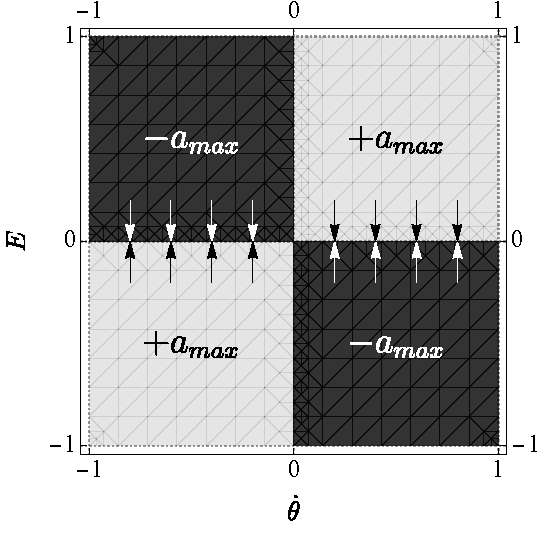
\includegraphics[width=\textwidth]{assets/energy-control1}
        \caption{$\cos\theta < 0$}
    \end{subfigure}
    \hfill
    \begin{subfigure}[b]{0.48\textwidth}
        \centering
        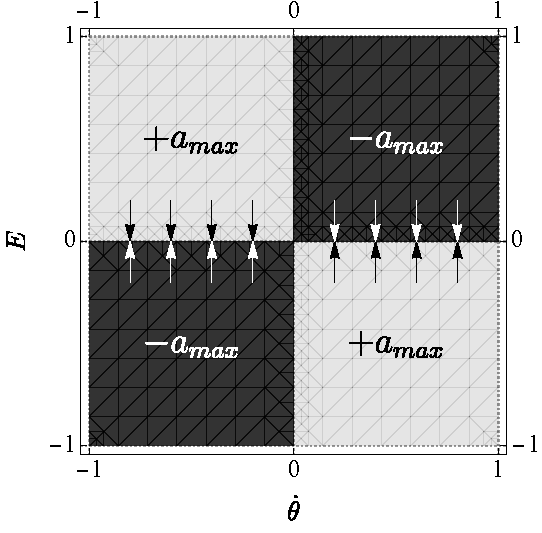
\includegraphics[width=\textwidth]{assets/energy-control2}
        \caption{$\cos\theta > 0$}
    \end{subfigure}
    \caption[Swing-up con funzione segno]{Strategia di swing-up con funzione segno.
    Nel grafico, il colore indica l'intensità dell'accelerazione $a$: il bianco
    corrisponde a un accelerazione verso destra e il nero ad un accelerazione verso sinistra.
    In modulo, l'accelerazione è sempre uguale. L'effetto del controllo, rappresentato dalle frecce, è
    di portare il sistema nella configurazione in cui $E = 0$.} %todo
    \label{fig:energy-control}
\end{figure}

\begin{figure}
    \centering
    \begin{subfigure}[b]{0.48\textwidth}
        \centering
        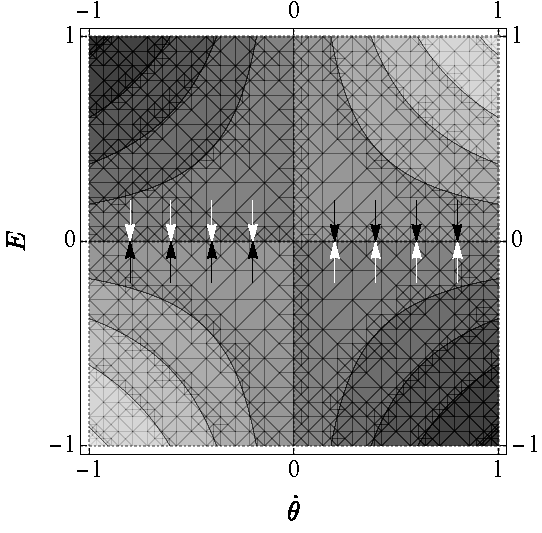
\includegraphics[width=\textwidth]{assets/energy-control3}
        \caption{$\cos\theta < 0$}
    \end{subfigure}
    \hfill
    \begin{subfigure}[b]{0.48\textwidth}
        \centering
        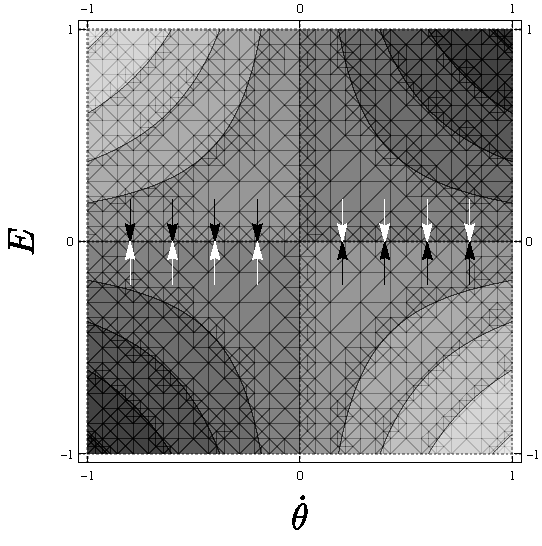
\includegraphics[width=\textwidth]{assets/energy-control4}
        \caption{$\cos\theta > 0$}
    \end{subfigure}
    \caption[Swing-up con tangente iperbolica]{Strategia di di swing-up con
    tangente iperbolica.
    Nel grafico, il colore indica l'intensità dell'accelerazione $a$: più è tendente al bianco, più è forte l'accelerazione verso destra e viceversa per il nero.
    L'effetto del controllo, rappresentato dalle frecce, è
    di portare il sistema nella configurazione in cui $E = 0$. I colori
    mostrano come questa strategia di controllo sia meno brusca della \eqref{eq:bang-bang}.} %todo
    \label{fig:energy-control-better}
\end{figure}

La funzione segno nella~\eqref{eq:bang-bang} la rende difficile da studiare
ed estremamente sensibile al rumore (la minima oscillazione costringe il motore
a passare istantaneamente da potenza zero a potenza massima).
Considero l'alternativa
\begin{equation}
    a = a_{\max} \tanh(E \dot \theta \cos \theta).
    \label{eq:control-strategy-tanh}
\end{equation}
Dimostro che la~\eqref{eq:lyapunov-energy} con $a$ definito come
nella~\eqref{eq:control-strategy-tanh} è una funzione di controllo di Ljapunov.
Uso la~\eqref{eq:dvdt}:
\begin{align*}
    \frac{dV}{dt} &=  E (-mal \dot \theta \cos \theta)\\
    &= -Eml \dot \theta \cos \theta \cdot a_{\max} \tanh(E \dot \theta \cos \theta). \numberthis\label{eq:a-ljapunov}
\end{align*}
ed è immediato verificare che la~\eqref{eq:a-ljapunov} è sempre negativa.
La~\eqref{eq:control-strategy-tanh} è rappresentata in \autoref{fig:energy-control-better}.

Concludo osservando che la strategia che ho mostrato in questo paragrafo
non tiene conto della posizione del carrello sulla rotaia.
È quindi necessario passare alla strategia di stabilizzazione
una volta che il pendolo ha raggiunto la verticale.
\section{Descrizione del sistema}
\label{sec:sistema-reale}
Il sistema è mostrato in \autoref{fig:foto-sistema}.
Per costruirlo ho usato componenti meccaniche ed elettroniche
disponibili commercialmente. Tutti i supporti di colore blu sono stati
realizzati con la stampa-3D. Segue una lista dettagliata di tutte le componenti.

\begin{figure}[H]
    \centering
    \fbox{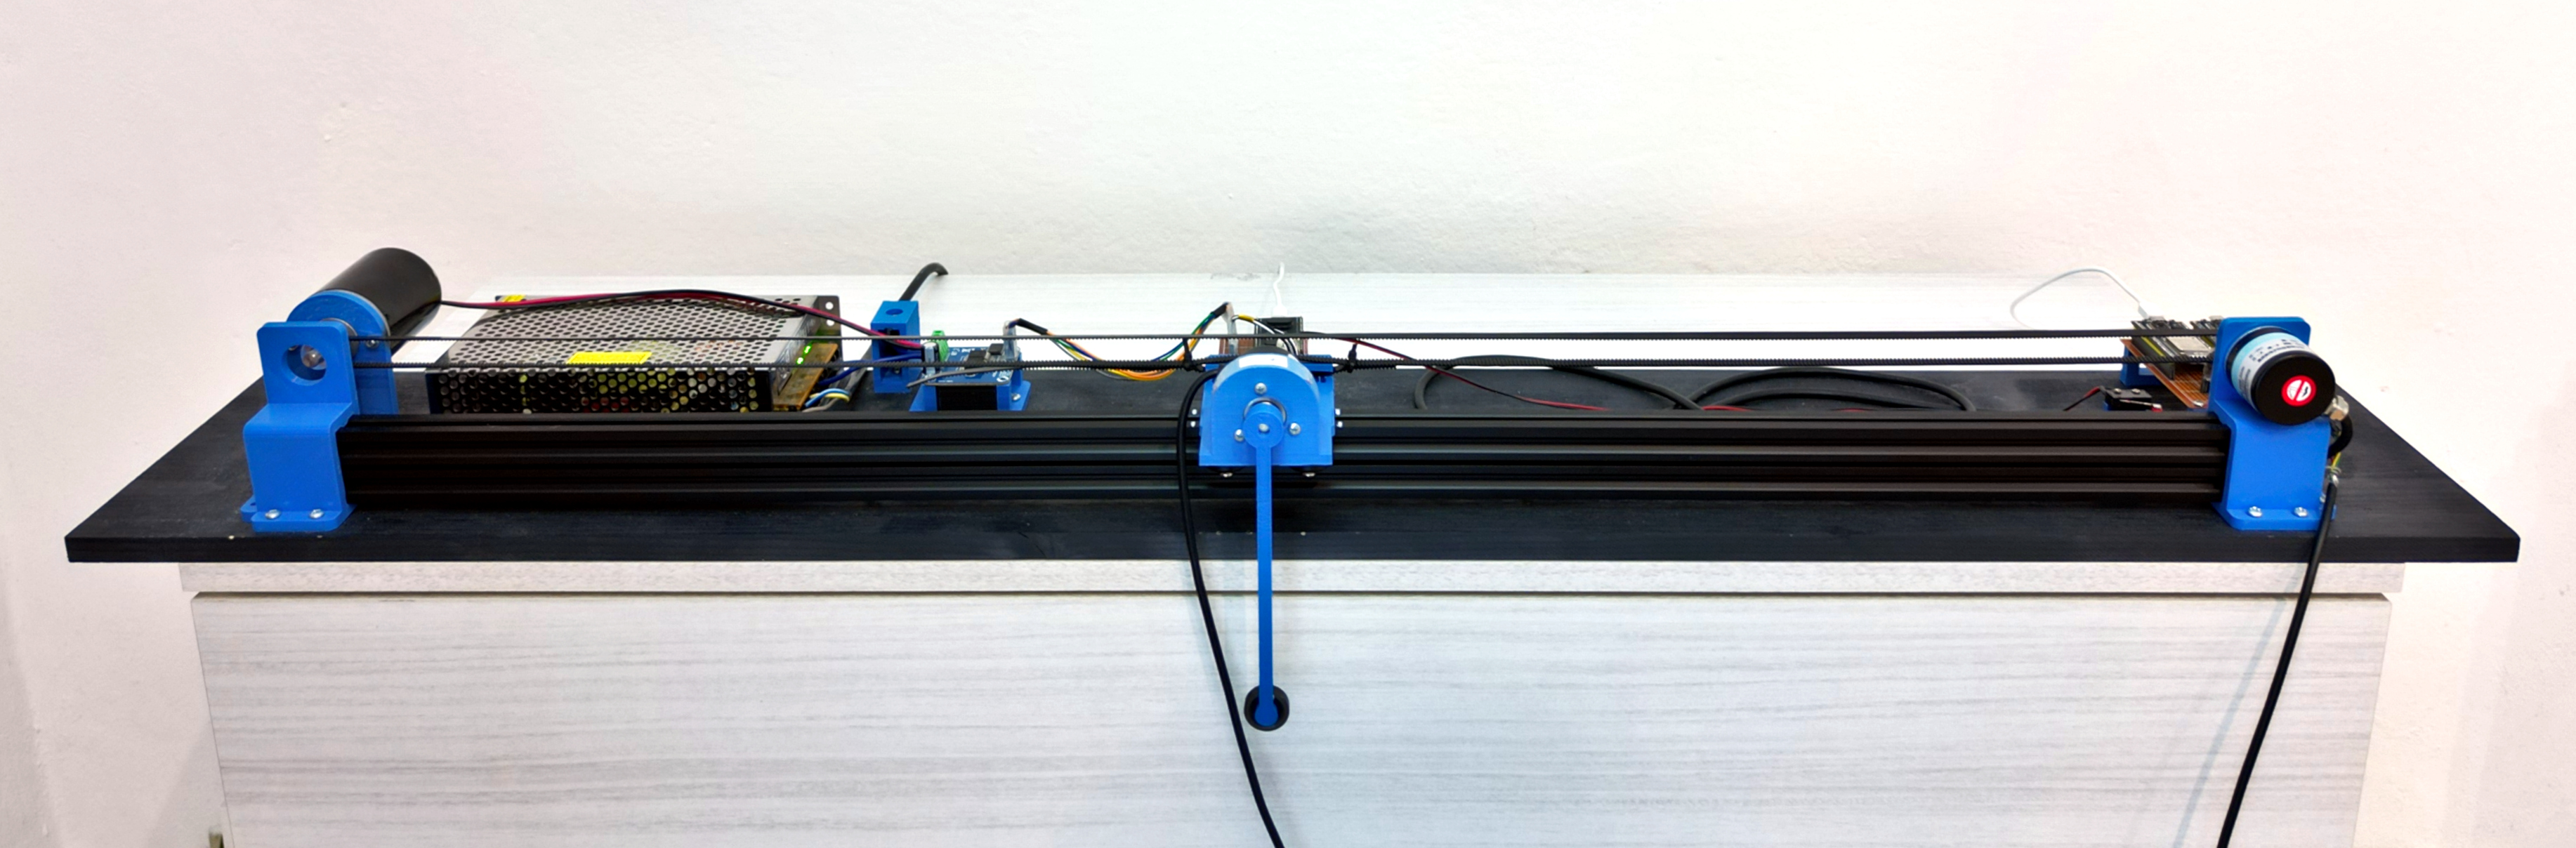
\includegraphics[width=.98\textwidth]{assets/pendolo-down}}
    \caption[Foto del sistema]{Foto del sistema che ho costruito, spento.}
    \label{fig:foto-sistema}
\end{figure}

\subsection{Componenti meccaniche}
\label{subsec:componenti-meccaniche}
Ho usato prevalentemente componenti standard di \emph{OpenBuilds},
%todo cite openbuilds.
assieme a supporti realizzati con la stampa-3D.
Tutte le componenti sono montate su una base di legno.

Il design meccanico è dettato dalla necessità di avere un vincolo
lineare per il carrello,
in modo da ridurre il più possibile tutti gli effetti non modellabili.
Il vincolo è dato da una rotaia, realizzata con un profilato in alluminio
\emph{V-Slot} lungo $1m$. Il carrello scorre sulla rotaia, supportato da
ruote \emph{Mini-V}. La forma delle ruote combacia con la forma del profilato, garantendo un movimento lineare, senza vibrazioni e con basso attrito.
Il dettaglio del carrello è riportato in \autoref{fig:dettaglio-carrello}.

\begin{figure}
    \centering
    \fbox{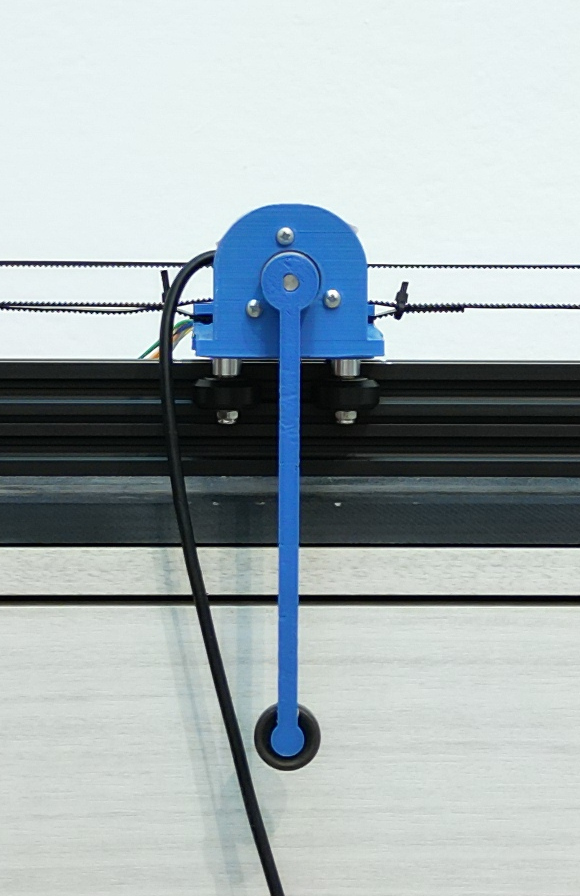
\includegraphics[width=.5\textwidth]{docs/report/assets/dettaglio-carrello}}
    %todo
    \caption[Dettaglio del carrello]{Dettaglio del carrello. Il pendolo è montato
    su un encoder, fissato al carrello tramite un supporto realizzato con la
    stampa-3D. Il carrello scorre sulla rotaia grazie alle ruote laterali.}
    \label{fig:dettaglio-carrello}
\end{figure}

Il carrello è collegato al motore tramite una cinghia dentata \emph{GT-2}.
La cinghia è di gomma con un cuore di metallo, in modo da resistere
alle deformazioni. La cinghia è mantenuta in tensione dal motore e da un
encoder rotativo, come mostrato in \autoref{fig:dettaglio-motore} e 
\autoref{fig:dettaglio-encoder}. Il motore è un modello \emph{XD-3420}
spazzolato, a corrente continua e con tensione nominale di $12V$.

Sul carrello è montato un secondo encoder rotativo,
che funge da perno per il pendolo. Il cavo collegato al secondo encoder è lasciato pendere ed il suo effetto sul sistema è trascurato.

\begin{figure}[h]
    \centering
    \fbox{\includegraphics[width=.8\textwidth]{docs/report/assets/particolare-motore}}
    %todo
    \caption[Dettaglio del motore]{Dettaglio di motore e alimentatore.
    Il motore è collegato al circuito \emph{H-Bridge} che, a sua volta, è collegato
    all'alimentatore. Un interruttore permette di disattivare il motore.
    Il motore è collegato direttamente alla cinghia.}
    \label{fig:dettaglio-motore}
\end{figure}
\begin{figure}[h]
    \centering
    \fbox{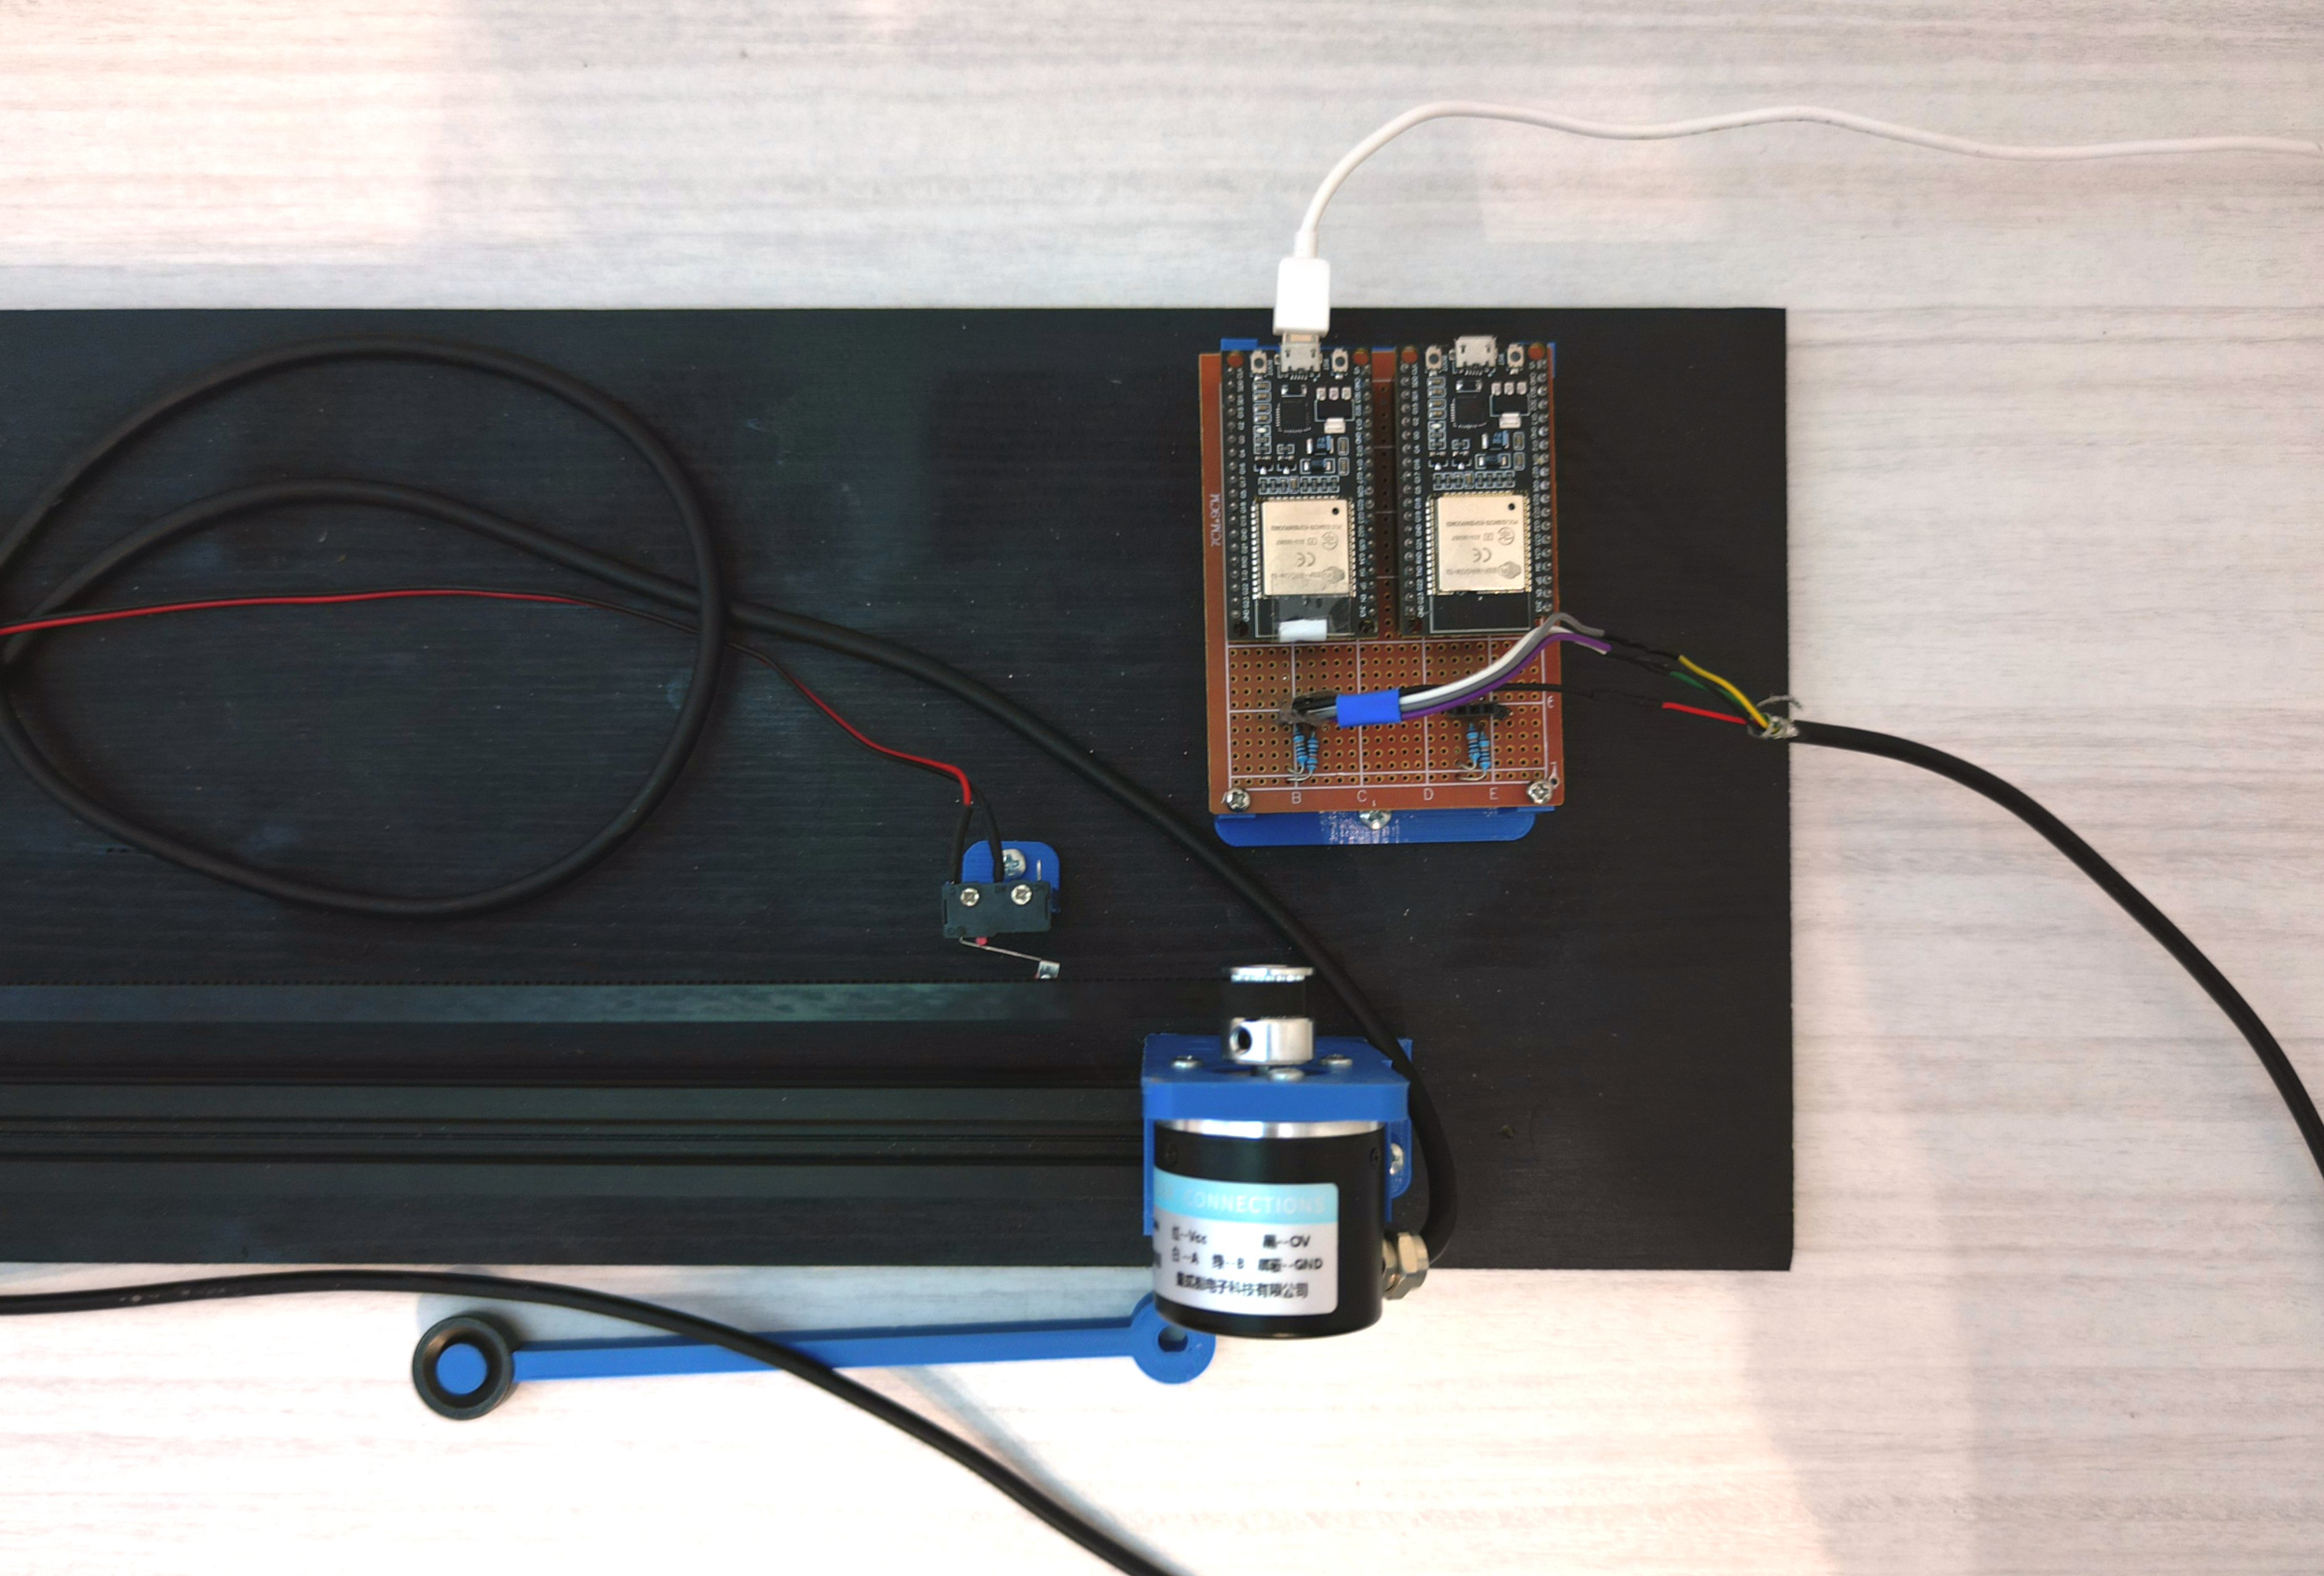
\includegraphics[width=.8\textwidth]{docs/report/assets/angle-sensor}}
    %todo
    \caption[Dettaglio encoder]{Dettaglio dell'encoder che misura la posizione.
    La cinghia è tenuta in tensione dall'encoder.
    In alto sono visibili due microcontrollori
    \emph{ESP-32}; solo uno di questi è utilizzato.
    }
    \label{fig:dettaglio-encoder}
\end{figure}


\subsection{Componenti elettroniche}
\label{subsec:componenti-elettroniche}

I sensori a cui il sistema ha accesso sono due encoder ottici\footnotemark rotativi,
modello \emph{LPD3806}. Il primo (\autoref{fig:dettaglio-carrello}) misura langolo del pendolo,
il secondo (\autoref{fig:dettaglio-encoder}la posizione del carrello.
Gli encoder sono incrementali, quindi devono essere azzerati manualmente
ogni volta che si avvia l'esperimento.

\footnotetext{
    Un encoder ottico rotativo è formato da un disco opaco su cui sono
    presenti delle fessure radiali. Una fotocellula è posta ai lati del disco
    e invia un impulso elettrico ogni volta che rileva una fessura. Una
    seconda fotocellula opera allo stesso modo, ma è posizionata in modo che il
    suo segnale sia sfasato rispetto alla prima. Confrontando i segnali delle due
    fotocellule, è possibile ricavare la direzione di rotazione.
}

I dati dei sensori sono letti da due microcontrollori \emph{ESP-32}.
%todo reference pls
I due microcontrollori comunicano usando la tecnologia \emph{ESP-NOW}.
%todo anche qui refenrece
Gli \emph{ESP-32} sono dotati di un microprocessore dual-core. Questo mi
permette di riservare un core in ciascun microcontrollore solamente per contare
gli impulsi ricevuti dal rispettivo encoder. Il secondo core è usato, in un caso,
per comunicare i dati all'altro microcontrollore e, nell'altro, per ricevere i dati
e inviare il segnale di controllo al motore. I due microcontrollori sono mostrati
in \autoref{fig:dettaglio-controller} e in \autoref{fig:dettaglio-encoder}.

\begin{figure}[h]
    \centering
    \fbox{\includegraphics[width=.8\textwidth]{docs/report/assets/particolare-controller}}
    %todo
    \caption[Dettaglio controller]{Dettaglio
    del microcontrollore che controlla il motore.
    Si vede il collegamento con il circuito
    \emph{H-Bridge}.}
    \label{fig:dettaglio-controller}
\end{figure}

Il motore è alimentato da un alimentatore da $12V$ (\autoref{fig:dettaglio-motore}).
La corrente passa in un circuito a \emph{H-Bridge}, modello \emph{BTS7960},
che permette di cambiare potenza e direzione di rotazione del motore.
La potenza del motore è regolata da un microcontrollore, collegato all'\emph{H-Bridge}, tramite \emph{PWM}\footnotemark. I due microcontrollori sono alimentati da due alimentatori esterni da $5V$. Internamente il sengale \emph{PWM} è rappresentato da un
numero a $8$-bit; il range di valori ammessi per $u$ è quindi $[0, 255] \subset N$.


\footnotetext{
    \emph{PWM} sta per \emph{Pulse Width Modulation}. La tecnica consiste
    nell'inviare al motore una corrente sotto forma di onda quadra.
    L'onda può avere valori di $0V$ o $12V$ e, variando la percentuale di tempo
    che l'onda passa a $12V$, si può variare la potenza del motore.
    Nel mio caso la frequenza dell'onda si è rilevata poco influente sul
    risultato; io ho fissato la frequenza a $500Hz$.
}

Nel sistema non è presente un sensore di corrente in ingresso al motore.
Questo è il motivo per cui nel paragrafo~\ref{subsec:modello-motore} ho limitato
il mio studio al regime stazionario.

\subsection{Dati in uscita dai sensori}
Il microcontrollore che si occupa di controllare il motore riceve i dati
aggiornati dei sensori ogni $2ms$.
Per evitare di sovraccaricare il processore, il segnale di controllo
del motore viene aggiornato una volta ogni $5ms$ e i dati del sistema vengono
trasmessi a un eventuale computer collegato solo una volta ogni $25ms$.
Nonostante il segnale di controllo non sia continuo, l'intervallo temporale
tra un segnale e il successivo è abbastanza piccolo da poterlo approssimare come
tale. Se così non fosse, sarebbe necessario discretizzare
il modello secondo la la~\eqref{eq:bdequalsint} .

Preciso inoltre che, mentre i dati per $q$ e $\theta$ sono presi esattamente
come escono dai sensori, per i dati di $\dot q$ e $\dot \theta$ viene presa
la media mobile degli ultimi tre punti, in modo da ridurre il rumore.
\section{Stima dei parametri del sistema nel mondo reale}
Non tutti i parametri descritti in tabella \ref{tab:parametri} sono calcolabili facilmente. In particolare, mi sono sconosciuti:
\begin{itemize}
    \item I parametri del motore.
    \item Il momento d'inerzia del pendolo.
\end{itemize}
In questa sezione userò i dati raccolti dal sistema reale per ottenere una stima di questi parametri.
Anche qui, mi conviene separare lo studio del pendolo dallo studio del motore.

\subsection{Parametri del pendolo}
La massa del pendolo si può misurare direttamente con una bilancia.
Anche la posizione del centro di massa è facile da trovare, bilanciando
il pendolo su un supporto e misurando la distanza tra questo e l'estremità.
Il momento d'inerzia è difficile da calcolare direttamente, visto che il
pendolo che ho usato è stato realizzato tramite la stampa 3d e, di conseguenza,
è estremamente disomogeneo all'interno; si può ricavare misurando
il periodo $\tau_{osc}$ di oscillazione del pendolo.
L'equazione del moto, nel regime delle piccole oscillazioni, è:
\begin{equation*}
    J \ddot \theta = mgL \sin \theta \approx mgL \theta
\end{equation*}
da cui
\begin{align}
    \omega &= \sqrt{\frac {m g L} J},\\
    \tau_{osc} &= \frac{2\pi}\omega = 2\pi \sqrt{\frac J {mgL}}.
    \label{eq:tau-osc}
\end{align}
La~\eqref{eq:tau-osc} permette di ricavare $J$ e fornisce una scala
di tempo per il sistema.


\subsection{Parametri del motore}
\label{subsec:parametri-motore}
Per determinare i parametri del motore, osservo come si comporta il sistema del solo
carrello, quando applico una \ddp $u$ costante ai capi del motore.
L'equazione che regola il comportamento del motore è la \eqref{eq:caratteristica-motore}.
Se scollego il pendolo dal carrello, l'espressione per la forza $f$
esercitata dal motore è data dalla legge di Newton:
\begin{equation}
    f = M \ddot q.
    \label{eq:newton-motore}
\end{equation}
Ora considero la sostituzione
\begin{equation}
    \begin{aligned}
    \dot q \mapsto v \\
    \ddot q \mapsto \dot v
    \end{aligned}
    \label{eq:sostituzione-motore}
\end{equation}
e inserendo \eqref{eq:newton-motore} e\eqref{eq:sostituzione-motore} dentro a \eqref{eq:caratteristica-motore}
ottengo l'equazione di una legge esponenziale:
\begin{equation*}
    \dot v = \frac{u - B v} {Am}.
\end{equation*}
Fisso la condizione iniziale $v(0) = 0$ e ottengo la soluzione:
\begin{equation}
    v(t) = \frac u B \left(1 - e^{-\frac B {Am} t}\right).
    \label{eq:equazione-fit-motore}
\end{equation}
I parametri $A$ e $B$ sono costanti quindi, variando $u$, mi aspetto di trovare
una famiglia di curve con cui fittare la \eqref{eq:equazione-fit-motore}.

In questa trattazione ho trascurato l'attrito tra carrello e rotaia.
Visto che il carrello scorre sulla rotaia attraverso dei cuscinetti,
l'attrito si può approssimare come costante.
Nel paragrafo ?? \todo{ref sezione risultati} mostrerò che in effetti questo attrito
è trascurabile.
\todo {traduci?}
Non è trascurabile invece il \emph{cogging torque} $\tau_c$ del motore,
dovuto all'interazione tra i magneti permanenti e le armature. $\tau_c$ ha
l'andamento descritto in figura \ref{fig:cogging} ed è predominante quando $\omega$ è
piccola.
L'approccio che ho usato per ridurne l'effetto è descritto nel paragrafo ?? \todo{anche qui paragrafo}.

%fixme i have no idea what this does but i used it so that the figure next doesn't span across
the whole page.
\makeatletter
\setlength{\@fptop}{0pt}
\makeatother

\begin{figure}[t]
    \centering
    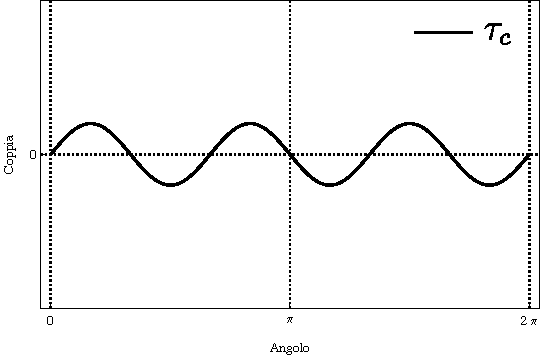
\includegraphics{assets/cogging-torque}
    \caption[Cogging torque]{Cogging toque del motore.}
    \label{fig:cogging}
\end{figure}

